\iffalse
	\section{Immediate}
	\begin{itemize}
		\item{} How many cases of obs that overlap asn obj that we should have seen
		\item{} Stay within $\pm$10~days of peak night
		\item{} how many observations dont have an entry in ddt file and why
		\item{} use log files
		\item{} ~~~column 12,13 are fitted RA and Dec
		\item{} ~~~if these and magzeropoint are 0 then theres no match due to failed observation
		\item{} ~~~if ra dec mzp do exist, then it should be in the ddt file
	\end{itemize}
\fi

\section{Expected Observations}\label{sec:expobs}
{\bf Rename section}
\iffalse
 ASASSN reported the discovery of 385 Supernovae (SN) by October 11, 2016. \\
 100 SN have a dec lower than -30\\
 165 SN were observed by asn before ATLAS observations began\\

 65 SN ...\\
 50/65 never had any sky/time overlap with ATLAS\\
 14/65 were 57364 or before, and the reductions were not very good\\
 1/65 (maybe) was before the SNII exploded, or it was really faint\\
 This left us with a total of 96 SN
\fi


{\bf Necessary to define MJD?}\\
%The primary factors restricting ATLAS observations were horizon and date.

\indent With a declination (dec) limit of approximately $-30^{\circ}$, 100 SN were not 
%expected to show up in the ATLAS data. 
expected to be present in the ATLAS data.
%ASASSN reported another 165 SN before ATLAS was operational. 
ASASSN reported the discovery of another 165 SN before ATLAS began collecting data. 
These two sets do not exist independent of one another. 
%After eliminating objects that fell below a dec of $-30^{\circ}$ and those that 
%peaked before ATLAS was truly up and running, we were left with 161(=65+96) ASASSN SN.
After applying dec and MJD based restrictions and accounting for overlaps between 
these groups, 161 SN remained from the initial 385 reported by ASASSN. 
%%%
Another 65 SN peaked before ATLAS was truly operational, leaving 96 as potential candidates.
%Although data was being collected, ATLAS was not instantaneously operational.
%%%
% CHECK VALIDITY OF THIS
All 96 of these objects were found in the ATLAS data, resulting in a 100\% completion rate.
%All 96 of these objects were found in the ATLAS data, giving a 100\% completion rate.
{\bf CHECK VALIDITY OF THIS}\\
%%%
%50/65 never had any sky/time overlap with ATLAS
%14/65 were 57364 or before, and the reductions were not very good
%1/65 (maybe) was before the SNII exploded, or it was really faint
%~[...]Another 65 SN peaked before ATLAS was truly operational.
\indent The 65 SN that peaked before ATLAS was truly operational can be further broken down as follows.\\
%Of these 65, 14 were reported to peak by 57364. 
%14 SN were reported to peak by 57364;
%14 SN were reported to peak on or before 57364; time during which reduced 
%ATLAS data is considered unreliable.
Reported peak brightnesses occurring on or before 57364 accounts for 14 SN. 
During this time the ATLAS reduction process was still being refined, making 
any reduced data unreliable.
%Reduction of data, by the ATLAS pipeline, was unreliable before this date.
%Data reduced by the ATLAS pipeline was not good enough to trust before 57364.
%%Another 50 fell in regions that had no overlap, due to ATLAS observations patterns.
Another 50 SN fell in regions that had no overlap with ATLAS observations due 
to the pattern in which data was collected.
%Based on observation patterns, another 50 SN are not expected to have any overlap / to have been observed.
The final case was a Type II supernova (SNII).
%The final SN was a Type II. 
%SNII are notoriously short lived. This makes it likely that...
SNII are notoriously short lived; making it likely that ATLAS observed this region of the sky in the 
time surrounding the explosion, but not during the event.
%Due to the short nature of Type II events, it is likely ATLAS observed that region of the sky in the 
%time surrounding the explosion, but not during the event.




\section{Failed Matches}
\iffalse
	\begin{itemize}
		\item{} 25 don't have a match at all. This may be because we're now using a +/-10 day window instead of +/-25.
		\item{} 49 don't have a diff file
		\item{} 15 don't have a ddt file
		\item{} 67 don't have a match in the ddt file
	\end{itemize}
\fi

{\bf Remove subsection headings?}

%For the 96 SN that overlap in time and location, 850 total ATLAS 
We expect to see 96 of the ASASSN SN in ATLAS observations. 
This presents us with 850 overlap opportunities, using a 
$\pm10~day$ window. Of these, 694 observations were recorded 
and properly reduced. %leaving 156 failed matches

\noindent {\bf Why these matches failed can be broken up into four categories -- 
no match, no difference image, no ddt file, or no match within an existing ddt file. 
These cases are discussed in sections~\ref{sec:nomatch}--\ref{sec:noddtline}.\\
\cref{sec:nomatch}--\cref{sec:noddtline}}\\%the subsections below.}\\
\noindent {\bf Why these matches failed can be broken up into four categories, 
%each of which is discussed in the following subsections.
each of which is discussed in the subsections below.}\\

%%%
% Compact these subsections into one section here
%%%
%25 don't have any matches at all. Must fall outside the nominal $\pm10~day$ window.
%49 lack diff imgs
%No ddt files exist for any observations in the nights any single ddt wasn't generated; accounting for 15/850.
%There are 67 instances where a ddt file exists but is missing the desired object.

\subsection{No match}\label{sec:nomatch}
%25 don't have any matches at all. Must fall outside the nominal $\pm10~day$ window.
A total of 25 expected observations lack any matches with ATLAS data. These failed 
matches do not fall within the $\pm10~day$ window used.


\subsection{No diff file}
%\indent Matches that were missing difference images can be attributed to an error 
%in the pipeline. Properly differenced images for part of the night shows a 
%failure in the pipeline occurred during differencing. Such a failure will 
%be corrected once the data is re-reduced.
\indent Missing difference images account for 49 of the expected 850 observations. 
Matches that were missing difference images can be attributed to an error in the 
ATLAS pipeline. An error during differencing caused a break in the pipeline and no 
further images to be generated for that night. Such an error will be corrected once 
the data is re--reduced.
%Properly differenced images for part of the night shows a 
%failure in the pipeline occurred during differencing. Such a failure will be corrected once the data is re-reduced.
%Such cases, part of the night was differenced properly. 


\subsection{No ddt file}
\indent For matches that were completely missing a ddt file, ddt files were missing 
for the entire night. This accounts for 15 failed matches and will be corrected by 
the next round of differencing.
%This mistake will be corrected by the next round of differencing.

\subsection{No ddt Match}\label{sec:noddtline}
%\begin{itemize}
	%\item{} ~[A] 3 is at the edge and fuzzy, causing ATLAS to miss it
	%\item{} ~[B] 26 Objects are in reduced image but not in difference image.
	%\item{} ~[C] 3 Object fell on a portion of the image that wasn't differenced properly and is a white chunk.
	%\item{} ~[D] 17 set of fits/diff images contains nothing at the indicated x,y coordinates
	%\item{} ~[E] 6 bright host galaxy, faint in difference image...must have been missed by ATLAS during difference photometry
	%\item{} ~[F] 3 unusable reduced and differenced data
	%\item{} ~[G] 8 unusable differenced data
	%\item{} ~[H] 1 not on image
%\end{itemize}

%Of the 67 occurrences missing a line in the ddt file:
%1 is at the edge and fuzzy, causing ATLAS to miss it
%x Objects are in reduced image but not in difference image. 

{\bf \indent Of the total 850 expected matches, 67 do not show up in existing ddt files.}
%
%Observations made at the beginning or end of a night are exposed to more 
%ambient light, causing fluctuations in the sky background. Poor observation 
%conditions account for 3 of the 67 missing ddt lines
Nature constantly plays a role in collecting astronomical data. When 
observations are made at the beginning or end of a night, ambient light 
levels rise and sky background fluctuations. 3 of the 67 missing ddt 
lines can be attributed to poor observation conditions, brought on by 
clouds and increased levels of sky background.\\
%
%
\indent Errors during the image differencing process led to the loss of 8 
expected overlaps. Older differencing techniques caused entire portions 
of images to be lost, accounting for 3 failed matches.\\
%Previous differencing techniques also account for [G].
%
\iffalse
	%Outdated differencing procedures caused the ATLAS pipeline to miss\\
	%Outdated differencing procedures caused the ATLAS pipeline not to trigger on faint\\
	The ATLAS pipeline failed to trigger on faint objects. \\
	%Outdated differencing procedures give rise to less consistent backgrounds,\\
	\indent Outdated differencing procedures lead to less uniform backgrounds, 
	%making it harder to distinguish between faint objects and {\bf (residual noise?)}. 
	making it harder to identify faint objects. {\bf reword?} 
	Bight host galaxies cause SN to become extremely faint in difference images. 
	%Such occurrences caused the ATLAS pipeline to miss [E] matches, during the difference photometry stage.\\
	Such occurrences caused the ATLAS pipeline to miss 6 matches while preforming 
	photometry on the differenced images.
\fi
\indent There were 6 cases where bright host galaxies caused the SN to become extremely 
faint in the difference image. Outdated differencing procedures lead to less 
uniform backgrounds, making it harder to identify faint objects. {\bf reword?} 
While preforming photometric calculations, the ATLAS pipeline failed to trigger 
on these 6 faint objects.\\
%
%
%The PSF across an image can vary due to numerous reasons.\\
\indent There are various reason why the PSF across an image may vary.
Here, the major contributers are high levels of sky background and optical 
issues inherent to the ATLAS system. 
%When gone uncorrected, such issues give rise to distortion\\
%If the proper corrections aren't made, such issues give rise to distortion\\
If not properly corrected for, such issues cause observed objects to become distorted. 
%Distortion causes sharp edges to blur, making it harder for the ATLAS pipeline to identify these objects.\\
%Distortion causes sharp edges to become fuzzy, making it harder for the ATLAS pipeline to identify these objects.\\
%Distortion can cause the sharp edges of an object to become fuzzy, causing the ATLAS pipeline not to trigger on such objects.\\
%Distortion can cause sharp edges to become fuzzy, causing the ATLAS pipeline not to trigger on such objects.\\
Distortion can cause sharp edges to become fuzzy, resulting in the ATLAS pipeline 
failing to trigger on such objects. This accounts for 3 of the missing matches.
Objects that were only in reduced images, but not in differenced images account 
for 26 of the matches missing from the ddt files. Such instances arise when the 
object is fully subtracted during differencing, due to it existing in the wallpaper.
% This occurs when an onject is in the wall paper
As the wallpaper is an ongoing project, corrected future versions will not cause this issue.\\
{\bf ~[WORDING]}\\
%
%
\indent There were 17 cases in which the SN was not detecting in either the reduced or 
differenced image, indicating poor astrometry. Another possible explanation is 
bad photometry. If photometry is the issue, the SN explosions must have occurred 
outside the nominal $\pm10~day$ window.\\
%
%
\indent The final group of matches missing from the ddt files comes from an issue with 
the array dimensionality. Each image is saved as a matrix. The software that 
%determines the correspondence between x,y-pixel coordinates and the objects RA, dec 
determines the correspondence between pixel coordinates and each objects RA, dec 
assumes the captured image fully extended to the edges of the matrix.
%(Due to the way the detectors are aligned,)?\\
In practice, the edges of some collected data are not completely filled. 
{\bf When these unfilled frames overlap with consecutive images, the objects lie where they are expected.} 
%Inspection of isolated images show that not every image fully extends to the intended edges. 
Not every image fully extends to the intended edges. 
%Inspection of isolated images show that every image does not fully extend to the intended edges. 
For this isolated case, the 
image data ends above the bottom edge of the array. Although the object is expected 
to be there, it does not exist on this particular image.


%\begin{figure*}
\begin{figure}[H]%[h!]
  \begin{center}
\centerline{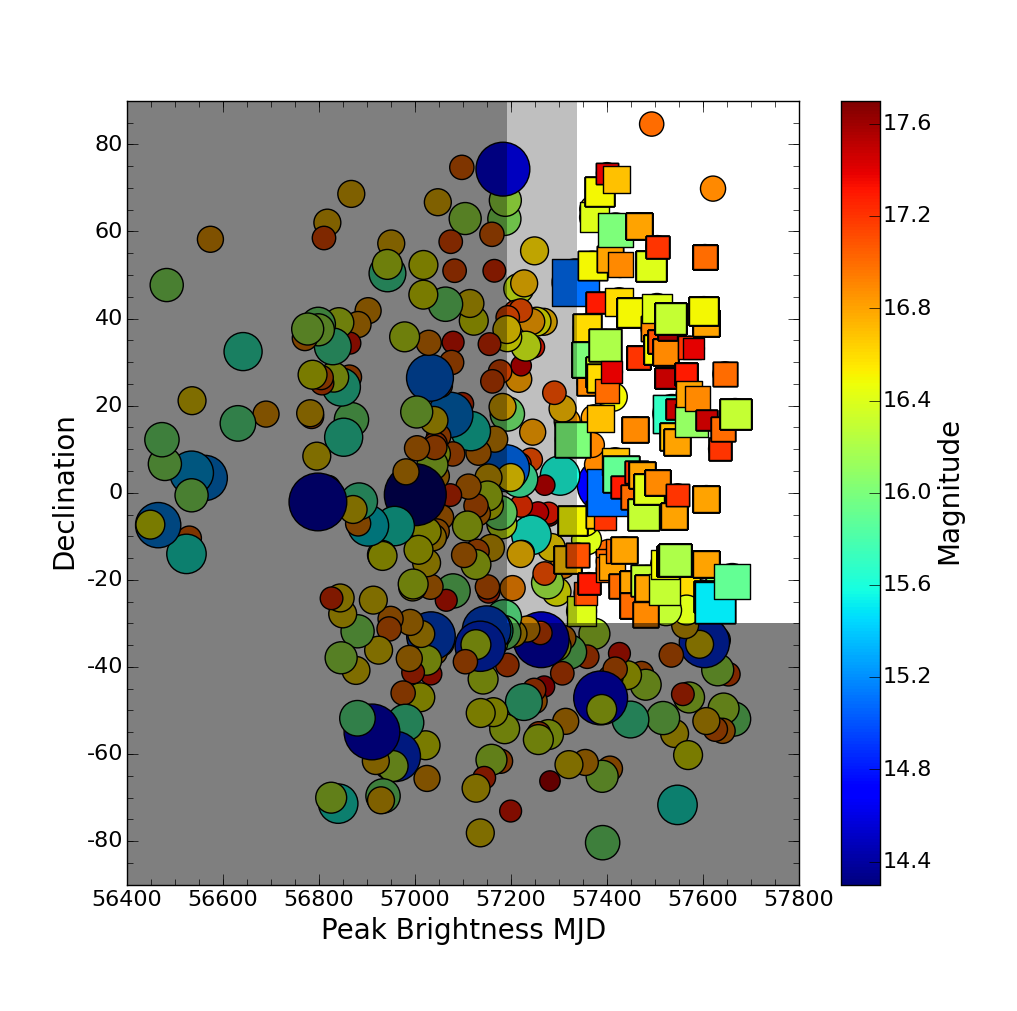
\includegraphics[width=3.35in]{figures/invert_mag.png}}
\caption{\it \small{ASASSN SN that do not have matches in ATLAS data are represented by circles. Squares show SN that were found in ATLAS observations. Regions that have a lower chance of containing SN have been covered in gray. Dark gray regions eliminate objects below the ATLAS observation limit of $-30\deg$ and those discovered before ATLAS was operational. The light gray region extends from ATLAS first night of collecting data up until 57364, when the reduction method was refined enough to produce usable data. Like the color, point-size represents magnitude.~\label{fig:dec_mjd}}}
  \end{center}
\end{figure}
%\end{figure*}


